\documentclass[conference]{IEEEtran}
% Default IEEE packages
\usepackage{cite}
\usepackage{amsmath,amssymb,amsfonts}
\usepackage{algorithmic}
\usepackage{graphicx}
\usepackage{textcomp}
\usepackage{xcolor}
\def\BibTeX{{\rm B\kern-.05em{\sc i\kern-.025em b}\kern-.08em
    T\kern-.1667em\lower.7ex\hbox{E}\kern-.125emX}}
    
% Additional packages
\usepackage{multirow}
\usepackage{tikz}


\newcommand{\xs}{-1}
\newcommand{\ys}{0.5}

% Tikz commands
\newcommand{\cube}[6]{  % 2 x-y, 3 dimensions, 1 color
        \begin{scope}[
        	shift={(#1, #2)},
			yslant=\ys ,xslant=\xs
            ]
            \filldraw[fill=#6] (0,0) rectangle (#3, #4);
            \draw[black] (0,0) rectangle (#3,#4);%marking borders
        \end{scope}
        \begin{scope}[
        	shift={(#1, #2)},
            yslant=\ys ,xslant=0
            ]
            \filldraw[fill=#6] (0,0) rectangle (#3, -#5);
            \draw[black] (0,0) rectangle (#3,-#5);%marking borders
        \end{scope}
        \begin{scope}[
        	shift={(#1, #2)},
            yslant=-\ys ,xslant=0
            ]
            \filldraw[fill=#6] (0,0) rectangle (-#4, -#5);
            \draw[black] (0,0) rectangle (-#4,-#5);%marking borders
        \end{scope}
}

\newcommand{\gridcube}[6]{  % 2 x-y, 3 dimensions, 1 color
        \begin{scope}[
        	shift={(#1, #2)},
            every node/.append style={
            yslant=0.5,xslant=-1},yslant=0.5,xslant=-1
            ]
            \filldraw[fill=#6] (0,0) rectangle (#3, #4);
            \draw[step=1, black!50] (0,0) grid (#3,#4); %defining grids
            \draw[black,very thick] (0,0) rectangle (#3,#4);%marking borders
        \end{scope}
        \begin{scope}[
        	shift={(#1, #2)},
            every node/.append style={
            yslant=0,xslant=0},yslant=0.5,xslant=0
            ]
            \filldraw[fill=#6] (0,0) rectangle (#3, -#5);
            \draw[step=1, black!50] (0,0) grid (#3,-#5); %defining grids
            \draw[black,very thick] (0,0) rectangle (#3,-#5);%marking borders
        \end{scope}
        \begin{scope}[
        	shift={(#1, #2)},
            every node/.append style={
            yslant=0,xslant=0},yslant=-0.5,xslant=0
            ]
            \filldraw[fill=#6] (0,0) rectangle (-#4, -#5);
            \draw[step=1, black!50] (0,0) grid (-#4,-#5); %defining grids
            \draw[black,very thick] (0,0) rectangle (-#4,-#5);%marking borders
        \end{scope}
}

\newcommand{\tikzcircle}[2][red,fill=red]{\tikz[baseline=-0.5ex]\draw[#1,radius=#2] (0,0) circle ;}%

    
\begin{document}

\title{Curvy DeepPicar}

\author{\IEEEauthorblockN{Patrick McNamee}
\IEEEauthorblockA{\textit{Department of Electrical Engineering and Computer Science} \\
\textit{University of Kansas}\\
Lawrence, KS \\
p678m854@ku.edu}}

\maketitle

\begin{abstract}

Convolutional Neural Networks (CNN) focus for vision based driving.
Neural network outputs tend to be very noise.
Previous work has shown that using the network outputs as a B\`ezier curves leads to smooth performances and outperform other network architectures. This work implements a CNN with B\`ezier curve outputs on a physical platform for vision navigation and evaluates the results.

\end{abstract}

\begin{IEEEkeywords}
machine learning, autonomous vehicles, embdedded platforms, guidance navigation and control
\end{IEEEkeywords}

\section{Introduction}

Modern car manufacturers are developing autonomous automobiles for future use in both civilian and military purposes. There are various complex environmental aspects that are required for consideration for autonomous agents to succeed in driving tasks such as sensors for object detection and localization, path planning, and state prediction for object avoidance \cite{kato2018}. These computational aspects traditionally rely on computational complex algorithms that may be too slow to implement on a real-time system. An alternative is to use neural networks which are universal approximators \cite{wang2021interval} to approximate the algorithms for a loss of functional accuracy but an increase in computational throughput. As such, neural networks have been frequently used for autonomous vehicle.

Usage of neural networks in autonomous ground vehicles has been around for decades with ALVINN being one of the first examples of vision-based navigation \cite{pomerieau-1989}. ALVINN used a 32 by 32 video input along with a 8 by 32 range finder input feed into a hidden layer of 29 units before the output layer of 46 units. The wheel steering angle was chosen based on the values of the 43 output units and ALVINN was quite successful at its various driving tasks. Modern implementations of autonomous cars, like the one developed by NVIDIA, are empowered by modern computational performance have since moved from the relatively simple network architecture used in ALVINN and currently use CNN which includes convolutional layers as well as significantly larger layers size \cite{bojarski2016end}. While these larger neural networks have allowed for more complex behavior of the autonomous agent, there are still issues that result from the nature of neural networks. Often the outputs of neural networks are rough in the sense  small manipulations on the input layer can produce drastically different outputs and there are no guarantees of output behavior in unexplored environments. Still, CNNs are potential methods to work towards fully autonomous driving and there are several implementation techniques to include them.

\subsection{Background}

There are various ways for CNN to be implemented for autonomous vision-based automobile navigation as reference in Figure \ref{fig:vb-steering}. The most direct method is to have the CNN take images and translate them into control inputs such as the steering angle or throttle as in \cite{bechtel2018}. While direct, this implementation is limited in that the controller is limited by the input rate of the camera systems as well as the network throughput implementation. It is also susceptible to network output roughness which can lead to high control jerk and unnecessarily fatigue physical components. This implementation of a direct controller is referred to in the rest of this work as image-to-point for translating a camera image into a point in the control dimensional space.

Two alternative implementations that are indirect schemes are navigational implementations and are implemented in DeepRacing \cite{trent2020iros}. Rather than directly control the car, the CNN outputs desired positions to navigate with a lower level control scheme closing the loop. There are two different ways to represent navigational points, discrete and continuous methods. A discrete method is simply to transform the input into a collection of ordered waypoints for navigation. However, CNN with rough outputs will still produce noisy outputs that may cause unwanted behavior. Additionally as the number of waypoints changes, the network architecture needs to be adjusted.

Rather than represent the waypoints or as discrete points, the waypoints can be represented as a continuous polynomial curves. B\`ezier curves $\mathbf{B}$ are useful representation as any polynomial of degree $d$ can be implemented with $d+1$ points $\mathbf{P}_k$ by \eqref{eq:bezier-curve} using a parameter $t$.

\begin{equation}
\label{eq:bezier-curve}
\mathbf{B}(t) = \sum_{k=0}^{d} \genfrac(){0pt}{0}{d}{k} (1-t)^{d-k}t^k \mathbf{P}_k \quad t\in [0, 1]
\end{equation}

This representation is advantageous as it can represent the same time window as the discrete waypoint representation but has an infinite number of points so the number of waypoints generated is not upper bounded. Additionally the waypoints are guaranteed to be smooth since they are on a polynomial curve and experimentally DeepRacing showed that this B\`ezier representation was the best performing network for CNN in simulated racing \cite{trent2020iros} but not any physical platform.

\begin{figure}[hbtp]
	\centerline{
	\begin{tikzpicture}
		% labeling
		\node at (-1.5,4) {a)};
		\node at (-1.5,2) {b)};
		\node at (-1.5,0) {c)};
		
		% Plot the basic images
		\foreach \y in {0,2,4}{
			\node at (0,\y) {\includegraphics[width=1.5cm,height=1cm]{..//figures/presentation/out-video-1-moment.jpg}};  % Image from camera
			\draw[blue, ultra thick, -latex] (0.8,\y) -- (1.45,\y);
			\filldraw[black, fill=black!60] (1.5,\y-0.25) rectangle node[white] {CNN} (2.5,\y+0.25);  % Neural Network
			\draw[red, ultra thick, -latex] (2.6,\y) -- (3.1,\y);
		}
		% Image-to-Point
		\draw (3.2,4) node[anchor=west] {$\theta_{\text{steering}} = 30^\circ$};
		% Image-to-Waypoints
		\draw[black, latex-latex] (3.2,1.5) -- (3.2, 2.5) node[anchor=south]{$y$};
		\draw[black, -latex] (3.2,2) -- (5,2) node[anchor=west]{$x$};
		\foreach \dx in {0.1,0.3,...,1.5}
			{\filldraw[red, fill=red] ( 3.2 + \dx , {2 - 0.15*pow(\dx, 2)} ) circle (1.5pt);}
		% Image-to-Curve
		\draw[black, latex-latex] (3.2,-0.5) -- (3.2, 0.5) node[anchor=south]{$\theta$};
		\draw[black, -latex] (3.2,0) -- (5,0) node[anchor=west]{$t$};
		\draw[red] (3.2,0) .. controls (3.75,0.5) and (4.25,-0.5) .. (4.9,-0.2);
		\draw[red] (3.2,0) circle (1.5pt);
		\draw[red] (3.75,0.5) circle (1.5pt);
		\draw[red] (4.25,-0.5) circle (1.5pt);
		\draw[red] (4.9,-0.2) circle (1.5pt);
		
	\end{tikzpicture}
	}
	\caption{Various Vision-Based Autonomous Steering Implementations. From top to bottom; a) image to direct control command, b) image to localized waypoints (\tikzcircle{2pt}), and c) image to curve using poles ({\color{red} $\circ$}).}
	\label{fig:vb-steering}
\end{figure}

While most work is focused on personal or racing automobiles, there have been implementations of vision-based navigation on small, radio-controlled cars. These vehicles are significantly cost-effective as research platforms and test embedded systems. Previous work at the University of Kansas has demonstrated implementing the DAVE-2 neural network architecture on a Raspberry Pi for a CNN image-to-point vision navigation system \cite{bechtel2018}. From a cost standpoint, the DeepPicar platform is ideal for testing a real implementation of a CNN with B\`ezier curve output although due to hardware and sensor limitations, an image-to-curve controller will need to used to compare the B\`ezier implementation of a controller against a standard image-to-point CNN controller.

\subsection{Motivations}

Previous work has shown the use of CNN outputting B\`ezier curves for navigation problems in simulated racing outperforms other techniques such as CNN outputting navigation waypoints or direct control networks \cite{trent2020iros}. However the simulation relies on position estimates which may not be feasible onboard small platforms or in environments with no direct position estimates and the B\`ezier curve outputs have, to the knowledge of the author, not been tested on a physical platform currently. Hence this work seeks to implement the a CNN outputting B\`ezier curves in a direct control scheme for navigating a track on the DeepPicar.

\section{Novel Contributions}

This work will implement a CNN outputting B\`ezier control curves for an embedded autonomous automobile platform for course navigation which has not been tested before on a physical platform. This new implementation will be tested against a standard CNN with direct control output as used in previous work \cite{bechtel2018} on the same physical platform.

\section{Convolutional Neural Networks}

\begin{figure*}[htbp]
	\centerline{
		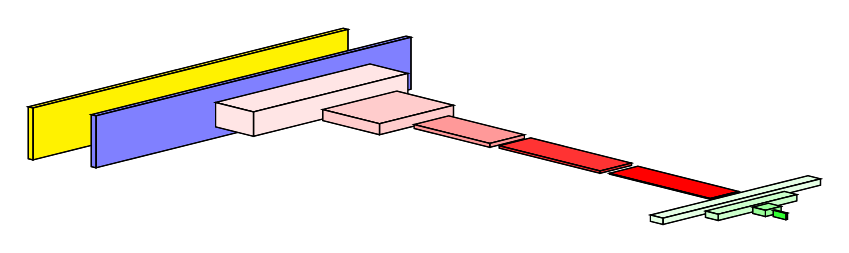
\begin{tikzpicture}[yscale=0.01, xscale=0.02]
		\cube{0}{0}{200}{3}{66}{yellow}
		\cube{40}{-10}{200}{3}{66}{blue!50}
		\cube{140}{-5}{98}{24}{31}{red!10}
		\cube{220}{-20}{47}{36}{14}{red!20}
		\cube{290}{-45}{22}{48}{5}{red!40}
		\cube{360}{-80}{20}{64}{3}{red!80}
		\cube{430}{-115}{18}{64}{1}{red}
		\cube{400}{-140}{100}{8}{8}{green!10}
		\cube{435}{-135}{50}{8}{8}{green!20}
		\cube{465}{-130}{10}{8}{8}{green!40}
		\cube{478}{-134}{1}{8}{8}{green!80}
		\end{tikzpicture}
	}
	\caption{Visualization of DAVE-2 Neural Network \cite{bojarski2016end}. Yellow is an input image, blue is the regularization layer, red is a convolution layer, and green is a dense layer. Dense layers are exaggerated for viewing and flattening omitted.}
	\label{fig:dave-2}
\end{figure*}

The CNNs are based off of the DAVE-2 CNN architecture from NIVIDIA \cite{bojarski2016end} and is shown in Fig. \ref{fig:dave-2}. Previous work has been implemented on a Raspberry Pi for the DeepPicar \cite{bechtel2018} and this work will use the same implementation as \cite{bechtel2018} to form a direct comparison with previous implementations. The input to the CNN is a Playstation Eye Camera which generates $320\times 240$ frames which are resized to $200\times 66$ to match the DAVE-2 inputs. Inside the CNN, the image is normalized across the image width, height, and channels before passing though multiple convolution layers. Layers 2, 3, and 4 use $5\times 5$ kernels with a width and height stride of $(2,2)$ while layers 5 and 6 use $3\times 3$ kernels with a width and height stride of $(1,1)$. After layer 6, the network is flattened to dense layers whose layer width is reduced until a single output unit. The activation functions used for layers 2 through 10 are rectilinear linear units (ReLU) while the last layer uses a hyperbolic tangent function. These activation functions are consistent with implementations in previous work \cite{bechtel2018,bojarski2016end} but the use of ReLU for the hidden layers are consistent with proofs that neural networks are universal approximators \cite{HORNIK1989359} and the hyperbolic tangent allows for outputs to be bounded to match the automobiles steering wheel angle limits $ [\theta_{\min},\ \theta_{\max}] $ by a linear transformation.

\subsection{Training Datasets}


There are two publically datasets available to train radio-control autonomous cars for tracks. The first dataset is a realitively small dataset consisting of only 200 example images but has a continuous steering angle ranging \cite{tian2019} while the other dataset consists of 11,000 example images but only has wheel angles in the set $\lbrace -30^\circ,\ 0^\circ,\ 30^\circ \rbrace$ degrees. As the B\`ezier curves deal with continuous outputs, it would be more advantageous from a training perspective to attempt to use Data Augmentation to train the various CNN models on the first dataset and then evaluate the CNN models on the larger second dataset.



<<<Show images from the two data sets>>>

Describe the data augmentation attempt.

<<<Table describing data augmentation accuracy>>>

Describe how handling data in discrete controller.



\subsection{Image-to-Point CNN}

\begin{table}[htbp]
	\centering
	\caption{Image-to-Point Convolutional Neural Network Architecture}
	\begin{tabular}{|r|c|c|r|}
	\multicolumn{1}{c}{\bfseries Layer} & \multicolumn{1}{c}{\bfseries Layer Type} & \multicolumn{1}{c}{\bfseries Dimension} & \multicolumn{1}{c}{\bfseries Parameters} \\ \hline
	1 & Normalizer & $66 \times 200 \times 3$ & 79,200 \\
	2 & 2D Convolution ($5\times5$)& $31 \times 98 \times 24$ & 1,824 \\
	3 & 2D Convolution ($5\times5$)& $14 \times 47 \times 36$ & 21,636 \\
	4 & 2D Convolution ($5\times5$)& $5 \times 22 \times 48$ & 43,248 \\
	5 & 2D Convolution ($3\times3$)& $3 \times 20 \times 64$ & 43,248 \\
	6 & 2D Convolution ($3\times3$)& $1 \times 18 \times 64$ & 43,248 \\
	7 & Flattening & $1152$ & 0 \\
	8 & Dense & $100$ & 115,300 \\
	9 & Dense & $50$ & 5,050 \\
	10 & Dense & $10$ & 510 \\
	11 & Dense & $1$ & 11 \\ \hline
	\multicolumn{2}{c|}{} & Non-trainable & 79,200 \\
	\multicolumn{2}{c|}{} & Trainable & 252,219 \\ \cline{3-4}
	\multicolumn{2}{c|}{} & Total & 331,419 \\ \cline{3-4}
	\end{tabular}
\end{table}

Brief description of the model architecture and loss function used in training.
How data is scaled for this model.

\subsection{Image-to-Curve CNN}

\begin{table}[htbp]
	\centering
	\caption{B\`ezier Convolutional Neural Network Architecture}
	\begin{tabular}{|r|c|c|r|}
	\multicolumn{1}{c}{\bfseries Layer} & \multicolumn{1}{c}{\bfseries Layer Type} & \multicolumn{1}{c}{\bfseries Dimension} & \multicolumn{1}{c}{\bfseries Parameters} \\ \hline
	1 & Normalizer & $66 \times 200 \times 3$ & 79,200 \\
	2 & 2D Convolution ($5\times5$)& $31 \times 98 \times 24$ & 1,824 \\
	3 & 2D Convolution ($5\times5$)& $14 \times 47 \times 36$ & 21,636 \\
	4 & 2D Convolution ($5\times5$)& $5 \times 22 \times 48$ & 43,248 \\
	5 & 2D Convolution ($3\times3$)& $3 \times 20 \times 64$ & 43,248 \\
	6 & 2D Convolution ($3\times3$)& $1 \times 18 \times 64$ & 43,248 \\
	7 & Flattening & $1152$ & 0 \\
	8 & Dense & $100$ & 115,300 \\
	9 & Dense & $50$ & 5,050 \\
	10 & Dense & $4$ & 204 \\
	11 & Reshape & $4\times 1$ & 0 \\ \hline
	\multicolumn{2}{c|}{} & Non-trainable & 79,200 \\
	\multicolumn{2}{c|}{} & Trainable & 251,902 \\ \cline{3-4}
	\multicolumn{2}{c|}{} & Total & 331,102 \\ \cline{3-4}
	\end{tabular}
\end{table}

\begin{figure}
	\centerline{
		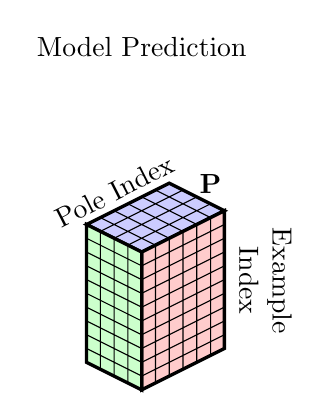
\begin{tikzpicture}[scale=0.175]
		\node at (0,12) {Model Prediction};
        % Top
        \begin{scope}[
            yshift=-83,every node/.append style={
            yslant=0.5,xslant=-1},yslant=0.5,xslant=-1
            ]
            \filldraw[fill=blue!20] (0,0) rectangle (6, 4);
            \draw[step=1, black] (0,0) grid (6,4); %defining grids
            \draw[black,very thick] (0,0) rectangle (6,4);%marking borders
        \end{scope}
        \begin{scope}[
            yshift=-83,every node/.append style={
            yslant=0,xslant=0},yslant=0.5,xslant=0
            ]
            \filldraw[fill=red!20] (0,0) rectangle (6, -10);
            \draw[step=1, black] (0,0) grid (6,-10); %defining grids
            \draw[black,very thick] (0,0) rectangle (6,-10);%marking borders
        \end{scope}
        \begin{scope}[
            yshift=-83,every node/.append style={
            yslant=0,xslant=0},yslant=-0.5,xslant=0
            ]
            \filldraw[fill=green!20] (0,0) rectangle (-4, -10);
            \draw[step=1, black] (0,0) grid (-4,-10); %defining grids
            \draw[black,very thick] (0,0) rectangle (-4,-10);%marking borders
        \end{scope}
        
        \draw (-2,1.5) node[rotate=27] {Pole Index};
        \node at (5,2) {$\mathbf{P}$};
        \draw (9,-5) node[rotate=-90, align=center] {Example\\ Index};
        \end{tikzpicture}
        \hspace{0.25in}
        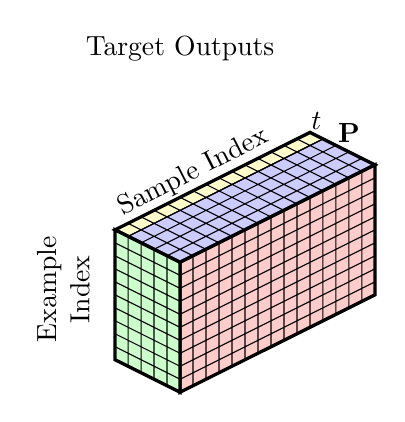
\begin{tikzpicture}[scale=0.165]
        \node at (0,13.5) {Target Outputs};
        % Top
        \begin{scope}[
            yshift=-83,every node/.append style={
            yslant=0.5,xslant=-1},yslant=0.5,xslant=-1
            ]
            \filldraw[fill=blue!20] (0,0) rectangle (15, 4);
            \filldraw[fill=yellow!20] (0,4) rectangle (15, 5);
            \draw[step=1, black] (0,0) grid (15,5); %defining grids
            \draw[black,very thick] (0,0) rectangle (15,5);%marking borders
        \end{scope}
        \begin{scope}[
            yshift=-83,every node/.append style={
            yslant=0,xslant=0},yslant=0.5,xslant=0
            ]
            \filldraw[fill=red!20] (0,0) rectangle (15, -10);
            \draw[step=1, black] (0,0) grid (15,-10); %defining grids
            \draw[black,very thick] (0,0) rectangle (15,-10);%marking borders
        \end{scope}
        \begin{scope}[
            yshift=-83,every node/.append style={
            yslant=0,xslant=0},yslant=-0.5,xslant=0
            ]
            \filldraw[fill=green!20] (0,0) rectangle (-5, -10);
            \draw[step=1, black] (0,0) grid (-5,-10); %defining grids
            \draw[black,very thick] (0,0) rectangle (-5,-10);%marking borders
        \end{scope}
        
        \draw (1,4) node[rotate=27] {Sample Index};
        \draw (-9,-5) node[rotate=90, align=center] {Example\\ Index};
        \draw (10.5,8) node {$t$};
        \draw (13,7) node {$\mathbf{P}$};
        \end{tikzpicture}
	}
	\caption{Implementation of Loss Function}
\end{figure}

Mention how the model is different from a standard image-to-point CNN.
How the interval is selected and used for training.
How the model can be interpreted

\subsection{Training}

Overview of training regiment

\section{Experiments}

Overview the  the quantitative approach for comparison with previous work.

\subsection{Model Accuracy}

	\begin{table}[btp]
        \centering
            \caption{Image-to-Point CNN Model (Acc: 20.45\%)}
            \begin{tabular}{|c|r|c|c|c|}
            \multicolumn{2}{c}{} & \multicolumn{3}{c}{\bfseries Model Predicted}\\\cline{3-5}
            \multicolumn{1}{c}{} & & \textbf{\textit{Left}} & \textbf{\textit{Center}} & \textbf{\textit{Right}}\\\hline
             \parbox[t]{2mm}{\multirow{3}{*}{\rotatebox[origin=c]{90}{\bfseries Record}}} & \textbf{\textit{Left}} & 48 & 31 & 21 \\\cline{3-5}
            & \textbf{\textit{Center}} & 156 & 156 & 188 \\\cline{3-5}
            & \textbf{\textit{Right}} & 54 & 136 & 205 \\\cline{3-5}\hline
            \end{tabular}
        \label{tab:i2p-acc}
    \end{table}
    
    \begin{table}[btp]
        \centering
            \caption{Image-to-Curve B\`ezier Model (Acc: 38.10\%) }
            \begin{tabular}{|c|r|c|c|c|}
            \multicolumn{2}{c}{} & \multicolumn{3}{c}{\bfseries Model Predicted}\\\cline{3-5}
            \multicolumn{1}{c}{} & & \textbf{\textit{Left}} & \textbf{\textit{Center}} & \textbf{\textit{Right}}\\\hline
             \parbox[t]{2mm}{\multirow{3}{*}{\rotatebox[origin=c]{90}{\bfseries Record}}} & \textbf{\textit{Left}} & 83 & 46 & 33 \\\cline{3-5}
            & \textbf{\textit{Center}} & 268 & 343 & 313 \\\cline{3-5}
            & \textbf{\textit{Right}} & 177 & 268 & 336 \\\cline{3-5}\hline
            \end{tabular}
        \label{tab:i2bc-acc}
    \end{table}

	    \begin{table}[tbp]
        \centering
            \caption{Image-to-Point B\`ezier Model (Acc: 66.75\%)}
            \begin{tabular}{|c|r|c|c|c|}
            \multicolumn{2}{c}{} & \multicolumn{3}{c}{\bfseries Model Predicted}\\\cline{3-5}
            \multicolumn{1}{c}{} & & \textbf{\textit{Left}} & \textbf{\textit{Center}} & \textbf{\textit{Right}}\\\hline
             \parbox[t]{2mm}{\multirow{3}{*}{\rotatebox[origin=c]{90}{\bfseries Record}}} & \textbf{\textit{Left}} & 60 & 111 & 9 \\\cline{3-5}
            & \textbf{\textit{Center}} & 48 & 667 & 261 \\\cline{3-5}
            & \textbf{\textit{Right}} & 13 & 223 & 608 \\\cline{3-5}\hline
            \end{tabular}
        \label{tab:i2bp-acc}
    \end{table}

<<<Video of Results>>>

\subsection{Physical Driving}

Outline of track used.
Mention how code was changed.
Give some results. 

\section{Results and Conclusions}

Mention that the most accurate model was found to be the B\`ezier CNN using only the first pole in an image-to-point set up.

Insert 

\section{Future Work}

The DeepPicar-v2 dataset is initially limiting; wheel angles are only three variations and there is a one-to-one correspondence between wheel angles and video frames. Curve fitting to noisy data best works with more sampling of points. Rather than constructing the dataset by forming corresponding pairs, have two threads of data collection. The first thread is for the camera at a nominal operational rate for image-to-point usage and the second thread is for 

\bibliographystyle{IEEEtran}
\bibliography{final-report}

\end{document}
